%% This is file `elsarticle-template-3-num.tex',
%%
%% Copyright 2009 Elsevier Ltd
%%
%% This file is part of the 'Elsarticle Bundle'.
%% ---------------------------------------------
%%
%% It may be distributed under the conditions of the LaTeX Project Public
%% License, either version 1.2 of this license or (at your option) any
%% later version.  The latest version of this license is in
%%    http://www.latex-project.org/lppl.txt
%% and version 1.2 or later is part of all distributions of LaTeX
%% version 1999/12/01 or later.
%%
%% The list of all files belonging to the 'Elsarticle Bundle' is
%% given in the file `manifest.txt'.
%%
%% Template article for Elsevier's document class `elsarticle'
%% with numbered style bibliographic references
%%
%% $Id: elsarticle-template-3-num.tex 165 2009-10-08 07:58:10Z rishi $
%% $URL: http://lenova.river-valley.com/svn/elsbst/trunk/elsarticle-template-3-num.tex $
%%

\documentclass[final,times,3p]{elsarticle}

%% Use the option review to obtain double line spacing
%% \documentclass[preprint,review,12pt]{elsarticle}

%% Use the options 1p,twocolumn; 3p; 3p,twocolumn; 5p; or 5p,twocolumn
%% for a journal layout:
%% \documentclass[final,1p,times]{elsarticle}
%% \documentclass[final,1p,times,twocolumn]{elsarticle}
%% \documentclass[final,3p,times]{elsarticle}
%% \documentclass[final,3p,times,twocolumn]{elsarticle}
%% \documentclass[final,5p,times]{elsarticle}
%% \documentclass[final,5p,times,twocolumn]{elsarticle}

%% PACKAGES

%% if you use PostScript figures in your article
%% use the graphics package for simple commands
%% \usepackage{graphics}
%% or use the graphicx package for more complicated commands
\usepackage{graphicx}
%% or use the epsfig package if you prefer to use the old commands
%% \usepackage{epsfig}
%% Hej Thomas, kan du se det? %og nu?
%% The amssymb package provides various useful mathematical symbols
\usepackage{amssymb}
%% The amsthm package provides extended theorem environments
%% \usepackage{amsthm}

%% The numcompress package shorten the last page in references.
%% `nodots' option removes dots from firstnames in references.
%% `nocompress' option prevent shortening of last page as
%% by default it will shorten.

\usepackage[nodots]{numcompress}
%% The lineno packages adds line numbers. Start line numbering with
%% \begin{linenumbers}, end it with \end{linenumbers}. Or switch it on
%% for the whole article with \linenumbers after \end{frontmatter}.
%% \usepackage{lineno}

%% natbib.sty is loaded by default. However, natbib options can be
%% provided with \biboptions{...} command. Following options are
%% valid:

%%   round  -  round parentheses are used (default)
%%   square -  square brackets are used   [option]
%%   curly  -  curly braces are used      {option}
%%   angle  -  angle brackets are used    <option>
%%   semicolon  -  multiple citations separated by semi-colon
%%   colon  - same as semicolon, an earlier confusion
%%   comma  -  separated by comma
%%   numbers-  selects numerical citations
%%   super  -  numerical citations as superscripts
%%   sort   -  sorts multiple citations according to order in ref. list
%%   sort&compress   -  like sort, but also compresses numerical citations
%%   compress - compresses without sorting

\usepackage{lineno}

%\usepackage{fleqn}
\usepackage{tikz}
\usepackage{pgfplots}
\usepackage{booktabs}
\usepackage{multirow}
\usepackage{amsmath}
\usepackage{nomencl}
\usepackage{framed} % Framing content
\usepackage{multicol} % Multiple columns environment
\usepackage{float}
\usepackage{rotating}
\usepackage{float}
\usepackage[pdftex,bookmarks=true]{hyperref}
\hypersetup{ 
    colorlinks,% 
    citecolor=black,% 
    filecolor=black,% 
    linkcolor=black,% 
    urlcolor=black 
} 
\usepackage{pgfplots, pgfplotstable}
\biboptions{square,sort&compress}

%% Contraction of references
\makeatletter
\def\NAT@spacechar{}
\makeatother

\renewcommand*\nompreamble{\begin{multicols}{2}}
\renewcommand*\nompostamble{\end{multicols}}

\RequirePackage{ifthen}

\renewcommand{\nomgroup}[1]{%
\ifthenelse{\equal{#1}{0}}{\item[\emph{Symbols}]}{
\ifthenelse{\equal{#1}{S}}{\item[\emph{Subscripts}]}{}}
\ifthenelse{\equal{#1}{P}}{\item[\emph{Superscripts}]}{
\ifthenelse{\equal{#1}{A}}{\item[\emph{Abbreviations}]}{}}
\ifthenelse{\equal{#1}{G}}{\item[\emph{Greek letters}]}{
\ifthenelse{\equal{#1}{O}}{\item[\emph{Others}]}}
}

\makeindex
\makenomenclature

\journal{Energy}

% Make the footnote space disappear for the first page (preprint and journal)
 
%\makeatletter
%\def\ps@pprintTitle{%
% \let\@oddhead\@empty
% \let\@evenhead\@empty
% \def\@oddfoot{}%
% \let\@evenfoot\@oddfoot}
%\makeatother

\begin{document}

\begin{frontmatter}

\title{Thermodynamic assessment of the Kalina Split cycle}

\author[]{Tuong-Van Nguyen\corref{cor}} \cortext[cor]{Principal corresponding author. Tel.: +45 4525 4129} \ead{tungu@mek.dtu.dk}
\author[]{Thomas Knudsen} 
\author[]{Ulrik Larsen} 
\author[]{Fredrik Haglind} 
\author[]{Brian Elmegaard}

\address{Section of Thermal Energy, Department of Mechanical Engineering, Technical University of Denmark,\\ Building 403, Nils Koppels All\'{e}, 2800 Kongens Lyngby, Denmark}

\begin{abstract}

The Kalina Split cycle is a thermodynamic process for converting thermal energy into electrical power, (i) using the ammonia-water mixture as working fluid, like a conventional Kalina cycle, and (ii) with a varying ammonia concentration during the heat extraction. This second feature results in an improved match between the heat source and working fluid temperature profiles, decreasing the entropy generation in the heat recovery system.  
The present work compares the thermodynamic performance of this power cycle with other configurations of the Kalina process, and investigates the impact of varying operating conditions. \textcolor{green}{The results indicate that the Kalina Split cycle with reheat presents an exergetic efficiency higher by 2.8\% points than a reference Kalina cycle with reheat, and by 4.3\% points without. The cycle performance is highly sensitive to its boundary conditions, varying by 9\% for a temperature variation of 30$^{\circ}$C for the cold reservoir and 100$^{\circ}$C for the stack. This analysis also pinpoints the large irreversibilities in the low-pressure turbine and condenser, which have an efficiency defect of 9.5-13\% and 7.2-13.7\%, respectively, and indicates a reduction of the exergy destruction by about 23\% in the heat recovery system.} 

\end{abstract}

\begin{keyword}
Kalina Split cycle \sep Energy analysis \sep Exergy assessment \sep Waste Heat Recovery 
\end{keyword}

\end{frontmatter}

%
%% Start line numbering here if you want
%%
\linenumbers

%% Main Text

%%%%%%%%% SECTION: INTRODUCTION %%%%%%%%%

\section{Introduction}
\label{sec:introduction}
	
%%%%%%%%% NOMENCLATURE %%%%%%%%%

\begin{table*}[!ht]
  \begin{framed}
  \footnotesize
    \printnomenclature
  \end{framed}
\end{table*}


\textcolor{red}{Waste heat recovery (WHR) systems are able to generate mechanical power and electricity without any fuel input and associated CO$_2$ emissions. Hence, with rising fuel prices and increased environmental awareness, motivation is growing for integrating these systems to improve the energy efficiency of various processes. An example is a WHR system for large marine engines in the present study. Organic Rankine cycles (ORC) and Kalina cycles are among the most frequently proposed alternatives to steam Rankine cycle WHR systems. At the scale of application studied in the present work, i.e. a net power output of 1-5 MW, both power cycles may be viable \cite{Tchanche20113963,Jonsson2001c}. Bombarda et al. \cite{Bombarda2010b} compared the two processes for a heat source temperature level of 346$^\circ$C and found that both cycles, when optimised, produced almost equal net power outputs. While the present study does not directly compare the ORC with the Kalina cycle, this work is based on the boundary conditions used in the work of Bombarda et al. \cite{Bombarda2010b}, in order to make comparisons about the power cycle performance for the same application.}

Energy can neither be created nor destroyed, and an energy analysis illustrates the energy transformations and flows throughout the system under study. On the opposite, exergy is not conserved in real processes, illustrating therefore the locations, causes and magnitudes of the thermodynamic irreversibilities taking place \cite{BejanAdrian;TsatsaronisGeorge;Moran1996,Bejan2006}. Exergy destruction also accounts for the additional exergetic fuel required because of the system imperfections \cite{Wall1988,Kotas1980,Kotas1980a,Kotas1995}. Several studies on the thermodynamic performance of the Kalina cycle exist. 

The present paper presents and evaluates a novel power generation cycle, called the Kalina Split cycle. This process is also based on the ammonia-water mixture as working fluid, like the conventional Kalina cycle, but is characterised by a varying ammonia concentration in the heat recovery system. This can result in a smaller entropy generation in the heat transfer process, and potentially in a higher exergetic efficiency of the complete power cycle. \textcolor{blue}{Shall we emphasise somewhere that we verify the statement smaller entropy generation in the boiler involves higher exergetic efficiency of the cycle?} This concept was briefly mentioned in the work of Kalina, and a system analysis was previously conducted by the same authors to identify the governing mechanisms of this process. The literature appears to contain little, if none, on the thermodynamic performance of such cycle, and this study aims at closing this gap, following these three objectives:

\begin{itemize}

	\item estimation of the cycle potential, in terms of energy and exergy efficiencies, compared to a conventional Kalina cycle, with and without reheat;
	\item analysis of the plant inefficiencies and of the exergy destruction trends;
	\item evaluation of the effect of the boundary conditions (heat source and cold reservoir temperatures) on the system performance.

\end{itemize}

Section \ref{sec:system_description} presents the design of the Kalina Split cycle system and the methods used in this work are reported in Section \ref{sec:methods}. The results are presented in Section \ref{sec:results} and are criticised further in Section \ref{sec:discussion}. Concluding remarks are outlined in Section \ref{sec:conclusion}.

\nomenclature[A]{ASPEN}{Advanced System for Process Engineering}
\nomenclature[A]{WHR}{waste heat recovery}
\nomenclature[A]{ORC}{Organic Rankine Cycle}
\nomenclature[A]{SC}{Split Cycle}
\nomenclature[A]{SUP}{superheated state}
\nomenclature[A]{SUB}{sub-cooled state}

%%%%%%%%% SECTION: SYSTEM DESCRIPTION %%%%%%%%%

\section{System description}
\label{sec:system_description} 

\subsection{Reference Kalina cycle}
\label{sec:kalina_cycle}

The Kalina cycle is similar in principle to the Rankine cycle, in which heat is supplied to a closed process loop and thermal energy is transformed into mechanical work. The main difference lies in the properties of the working fluid, which is an ammonia-water mixture in the Kalina cycle. This multicomponent mixture is zeotropic, which means that the vapor and liquid phases during evaporation do not present the same composition, At constant pressure, the boiling temperature changes during the heat transfer process, at the difference of pure substances, which have a constant evaporation temperature. 

This temperature glide allows a better matching between the temperature profiles of the heat source and receiver, causing therefore a smaller exergy destruction during the heat transfer process. The range of the temperature glide can be adjusted by modifying the ammonia and water fractions of the working solution, and the Kalina cycle may therefore be suitable for application in both low- and medium-temperature heat recovery applications.  

Several configurations of this thermodynamic cycle exist, and the layout considered in this work (Figure \ref{fig:kalina_cycle}) is the one presented in the study of Bombarda et al. \cite{Bombarda2010b} and was studied by Marston \cite{Marston1990,Marston1995} and El-Sayed \cite{El-Sayed1985}. The terms `rich' and `lean'  imply ammonia-rich and ammonia-lean in the rest of this work. Four different ammonia concentrations can be found in the conventional Kalina cycle: `very rich' (points 13 and 16), `rich' (points 1 to 5, and 18 to 21), `medium' (points 6 to 11, and 17) and  `lean' (points 12, 14 and 15). 

\begin{figure*}[htbp]
\centering
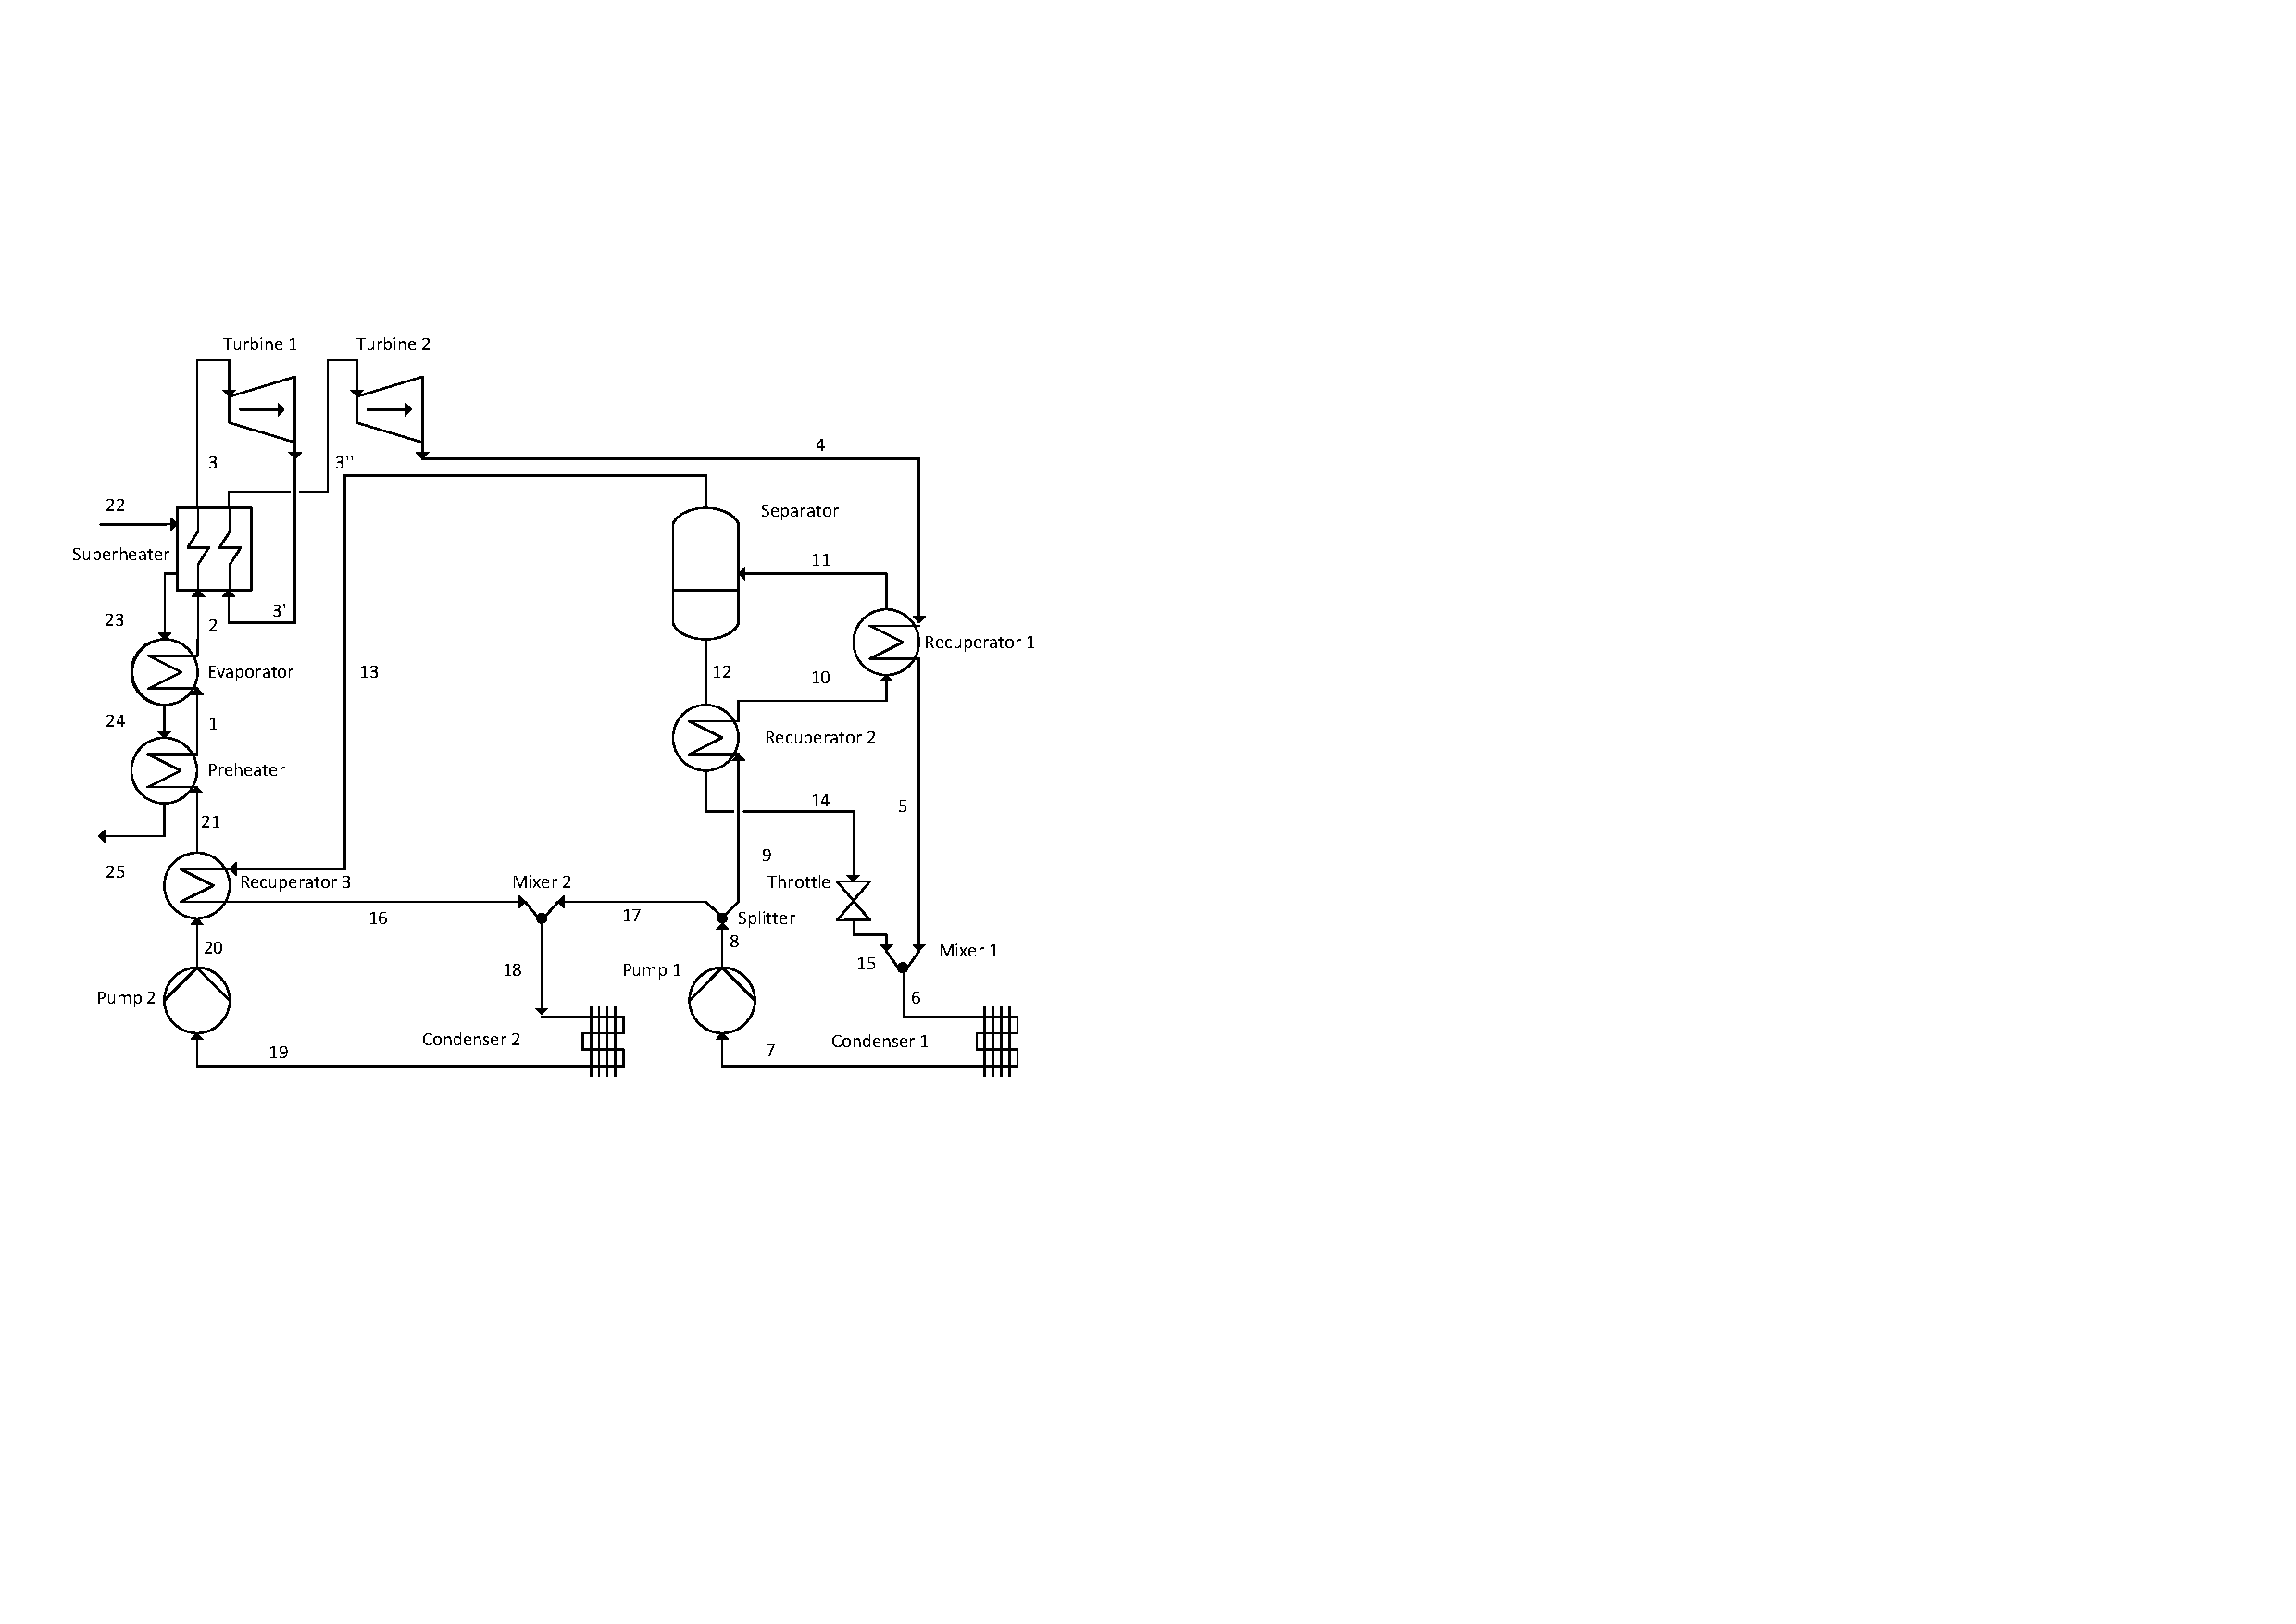
\includegraphics[width=0.9\linewidth]{Drawing_Kalina_Baseline.pdf}
\caption{Flowchart of the Kalina cycle process}
\label{fig:kalina_cycle}
\end{figure*}

The ammonia-rich mixture (1) enters the heat recovery system where it is evaporated (2) and superheated (3) by heat recovery. The working solution is expanded to a low pressure level (4), generating shaft work, and enters a first heat exchanger (Recuperator 1) where it is cooled and partially condensed (5). Reheat may be implemented, implying that the stream exiting the turbine re-enters the boiler at an intermediate pressure (3') and is heated (3'') to the same temperature as (3), before being expanded in a second turbine. Stream (5) is mixed with the lean solution (15), resulting in a working solution (6) with a higher condensing temperature. It is condensed (7), pumped to an intermediate pressure level (8), and split into two streams (9) and (17). Stream (9) is heated in a succession of two heat exchangers (Recuperator 2 and Recuperator 1) and enters (11) the vapour-liquid separator to form a lean liquid (12) and a very rich vapour (13). The lean liquid is cooled (14) and throttled to the lowest pressure level (15) of this power cycle.  The very rich vapour is cooled (16) and diluted with (17) into (18) in a second mixer. This working solution is condensed (19) and pumped to the highest pressure level (20), i.e. the boiler pressure, heated in two steps (21), and (1), by recovering heat from the waste heat source. 

\subsection{Kalina Split-cycle}
\label{sec:split_cycle}

The Kalina Split cycle is fundamentally similar to the Kalina cycle (Figure \ref{fig:split_cycle}), both using the ammonia-water mixture. The main difference lies in the change of ammonia concentration in the evaporation process, which involves a more complex splitting and mixing arrangement to achieve the desired ammonia concentrations. Five different concentrations can be found in the Kalina Split cycle and are denoted `very rich' (points 18, 19 and 26), `rich' (points 20 to 25, and 33) , `basic' (points 1 to 5), `lean' (points 27 to 32), and  `very lean' (points 11 to 16), in reference to their ammonia content. 

\begin{figure*}[htbp]
\centering
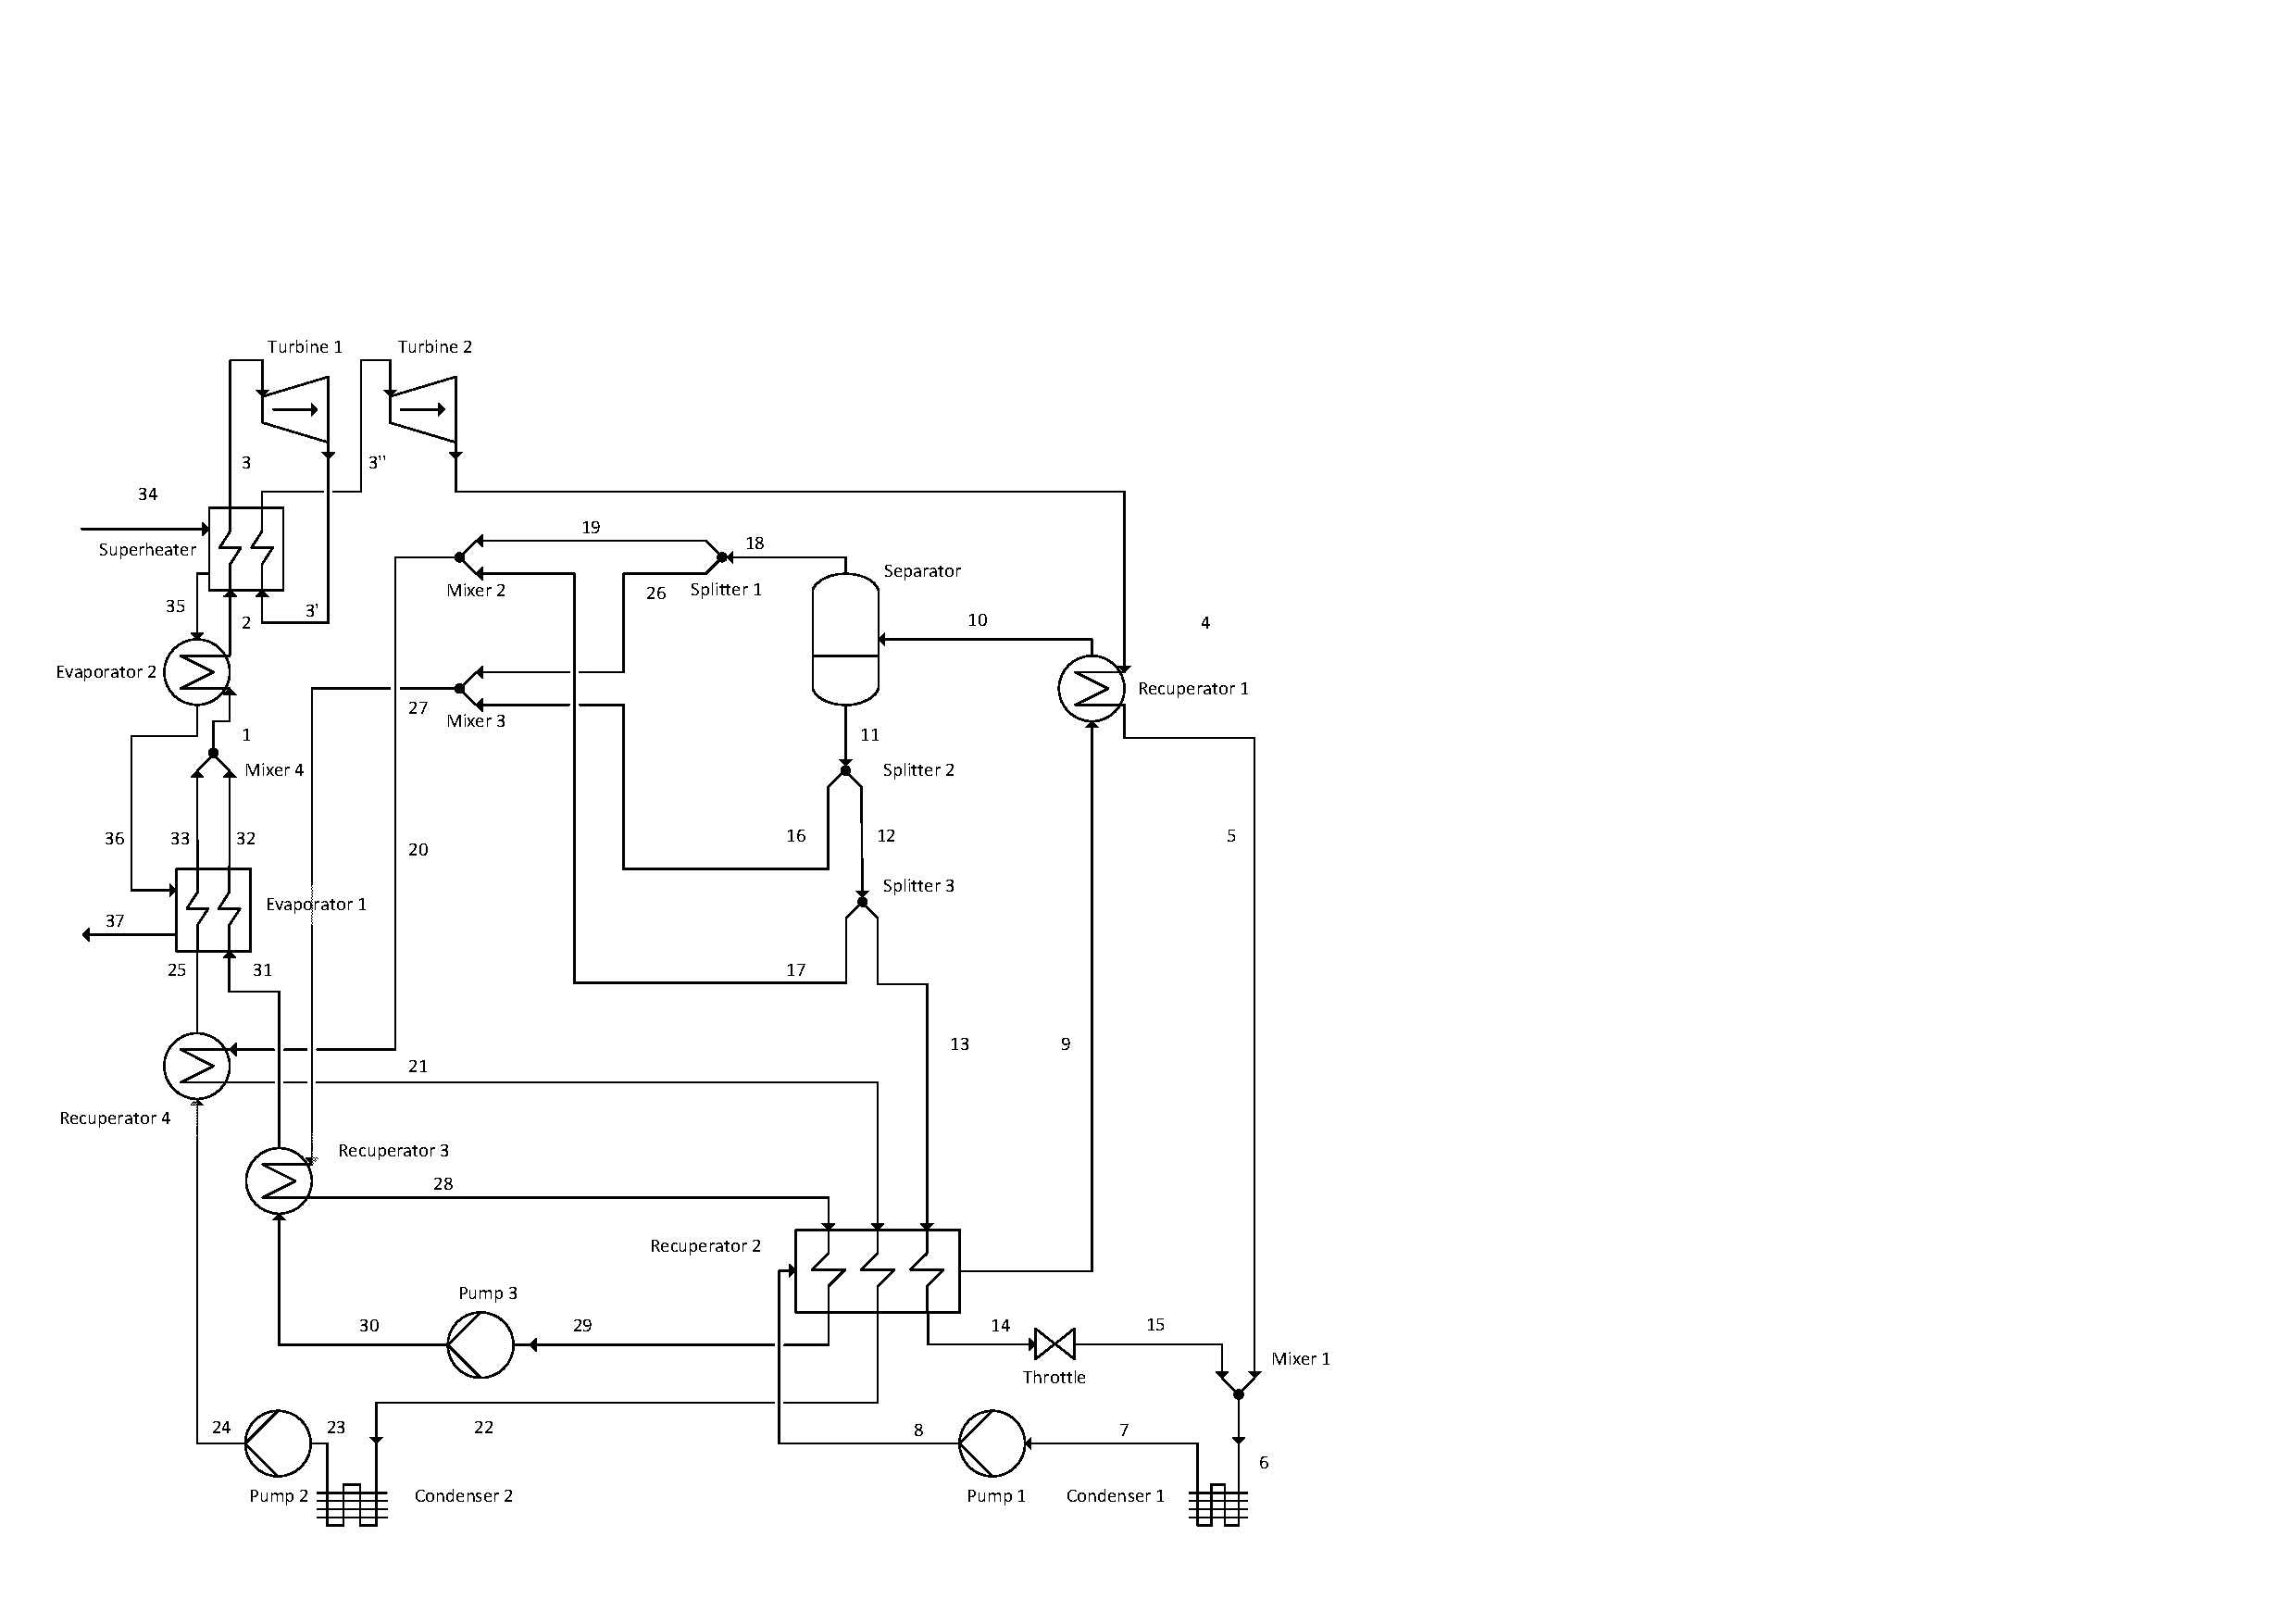
\includegraphics[width=1.0\linewidth]{Drawing_Kalina_Split.pdf}
\caption{Flowchart of the Kalina Split cycle process}
\label{fig:split_cycle}
\end{figure*}

At the difference of the Kalina cycle, two streams of different ammonia concentration enter the boiler (Figure \ref{fig:theory}, left), an ammonia-rich (25) and an ammonia-lean (31). The first one is fully evaporated (33) while the second one stays in liquid form, but is heated to its bubble point temperature (32), They are mixed into (1): the resulting solution is an ammonia-water solution in vapour-liquid equilibrium, which is evaporated (2) and superheated (3). 

The preheating stage is illustrated by the (25,31)--$T_{r,b}$ line: the lean and rich streams are sensibly heated to the bubble point temperature, recovering energy from the heat source. The dashed upper line $T_{r,b}$--$T_b$ illustrates the heat transfer-temperature path if the rich and lean streams enter the boiler as a single stream, as in the conventional Kalina cycle. The dashed lower line $T_{r,b}$--$T_{2a}$ represents the T -Q path if a single stream with the same ammonia concentration as the rich stream enters the boiler. \textcolor{blue}{What about the lean stream? I guess it would be under as it would not start yet to evaporate, but maybe we should write a bit on that too?} The full line $T_{r,b}$--$T_{1}$ corresponds to the Split Cycle configuration, with two streams of different concentrations. 

The difference between the paths $T_{r,b}$--$T_b$ and $T_{r,b}$--$T_{1}$ suggests that the Kalina Split cycle offers more flexibility, as the concentrations of the two streams entering the boiler can be adjusted to prevent a too small temperature difference between the heat source and receiver. The difference between the paths $T_{r,b}$--$T_{1}$ and $T_{r,b}$--$T_{2a}$ indicates that the split cycle configuration results in a better match of the enthalpy-temperature curves, and therefore in a smaller entropy generation in the boiler. In all cases, the minimum temperature difference, i.e. the pinch point location, is found in the evaporation process, i.e after the preheating and before the mixing of the rich and lean streams. 

\nomenclature[S]{r}{rich ammonia concentration} \nomenclature[S]{b}{bubble point}

This work assumes that the rich and lean streams are mixed at same temperature and pressure to reduce the entropy generation due to mixing effects. In addition, Kalina \cite{Kalina1986a} suggested that the rich stream should be at dew point conditions, while the lean stream should be at bubble point ones. The vapour and liquid phases of each stream are therefore at their equilibrium concentrations, which would minimise the entropy generation in the mixing process. However, such constraint fixes the mixing temperature, as the ammonia concentration of the lean and rich streams are interdependent. The actual mixing point has little influence on the overall performance of the system, since the pinch point is indeed located either at the bubble temperature of the ammonia-rich stream $T_{r,b}$--$T_{b}$ or at the outlet of the superheater $T_{3}$--$T_{34}$. 

\begin{figure*}[htpb]
\centering
\begin{tikzpicture}[scale=0.9]

\begin{axis}[xlabel={Accumulated heat transfer},
	ylabel={Temperature},
	axis lines*=left,
	legend pos=outer north east,
	no markers,
	xticklabels={,,},
	yticklabels={,,}
	]

\addplot [style=thick] table[x index=0,y index=1,col sep=space] {theory.data}; %split
\addplot table[x index=0,y index=1,col sep=space] {theoryHeatSource.data}; %heat source
\addplot [style=dashed] table[x index=0,y index=1,col sep=space] {theoryRich.data}; %rich alone
\addplot [style=dashed] table[x index=0,y index=1,col sep=space] {theoryComp.data}; %composite

\node[] at (40,1) {$25,31$}; 
\node[] at (100,22) {$T_{r,b}$};
\node[] at (50,50) {$T_{b}$};
\node[] at (200,60) {$1$};
\node[] at (300,70) {$2$};
\node[] at (270,45) {$2a$};
\node[] at (400,92) {$3$};
\node[] at (0,25) {$37$};
\node[] at (400,112) {$34$};

\end{axis}
\end{tikzpicture}
\hfill
\begin{tikzpicture}[scale=0.9]

\begin{axis}[xlabel={Rich stream (25) NH$_3$-concentration},
	%xmin=0.75, xmax=1.0,
	ymin=0.2,
	axis x line*=bottom,
	axis y line*=left,
	ylabel={Lean stream (31) NH$_3$-concentration},
	ylabel near ticks,
	legend style={legend pos=south west,font=\small, draw=none} ,
	]

\addplot [mark=triangle*, mark options={fill=black}] table[x index=0,y index=1,col sep=space] {data/bubbleDewPoints.txt};
\addlegendentry{Concentration}

\end{axis}

\begin{axis}[xlabel={},
	%xmin=0.75, xmax=1.0,
	ymin=100,
	axis x line*=bottom,
	hide x axis,
	axis y line*=right,
	ylabel={Mixing temperature ($^\circ$C)},
	ylabel near ticks,
	legend style={legend pos=south east,font=\small, draw=none} ,
	]

\addplot table[x index=0,y index=2,col sep=space] {data/bubbleDewPoints.txt};
\addlegendentry{Temperature}

\end{axis}
\end{tikzpicture}

\caption{Split Cycle Mechanisms: T-Q diagram of the heat recovery system (\emph{left}) and Temperature-NH$_3$ concentration dependency (\emph{right})}
\label{fig:theory}
\end{figure*}

\section{Methods}
\label{sec:methods}

\subsection{Baseline case}

This study builds on a baseline case adapted from the work of Bombarda et al. \cite{Bombarda2010b}, where the integration of a bottoming Kalina cycle is studied, using exhaust gases from diesel engines as heat source. The Kalina cycle is compared to the Kalina Split cycle, considering one reheat stage as a possible option (Table \ref{tab:system_baseline}).

\begin{table}[htbp]
\scriptsize
  \centering
  \caption{System parameters (baseline case)}
    \begin{tabular}{llr}
    \toprule
    Parameter & Description  & Value \\
    \midrule
     $T_{34}$ & Heat source inlet temperature & 346 $^{\circ}$C \\
     $T_{37}$     & Heat source outlet temperature & 127.7 $^{\circ}$C\\
     $T_{cw}$    & Cooling water inlet temperature & 25 $^{\circ}$C\\
     $T_{34}-T_{3}$  & Superheater approach & 16 $^{\circ}$C\\
     $\Delta T_{evap}$     & Minimum temperature difference (evaporators) & 21.9 $^{\circ}$C \\
     $\Delta T_{rec}$    & Minimum temperature difference (recuperators) & 5 $^{\circ}$C \\
     $\Delta T_{cond}$   & Minimum temperature difference (condenser) & 4.5 $^{\circ}$C \\
     $\eta_{t,pol}$    & Turbine polytropic efficiency & 70.5$\%$\\
     $\eta_{t,mec}$    & Turbine mechanical efficiency & 96$\%$\\
     $\eta_{pp}$    & Pump efficiency & 70$\%$\\
     $\eta_{dr}$  & Driver efficiency & 95$\%$\\
    \bottomrule
    \end{tabular}%
  \label{tab:system_baseline}%
\end{table}

\subsubsection{Modelling}

		\subsubsection{Simulation}
	
		\subsubsection{Validation}
			
	\subsection{Energy analysis}
	\label{subsec:energy_analysis}
		
	\emph{Energy} may be stored, transformed from one form to another and transferred between systems, but, as stated by the 1st law of thermodynamics, energy can neither be created nor destroyed. In open systems, energy can be transferred in or out of the system under study by streams of matter, heat and work. Neglecting the kinetic and potential energies, the energy rate balance at steady state is:
	
	\begin{equation}
	0=\sum_k \dot{Q}_{k}-\dot{W}_{cv} + \sum \dot{m}_{in} h_{in} - \sum \dot{m}_{out} h_{out}
	\end{equation}
	
	where $\dot{Q}_{k}$ and $\dot{W}_{cv}$ the time rates of energy transfer by heat and work. The convention adopted in this work is that $\dot{Q}\ge0$ indicates heat transfer to the system and $\dot{W}\ge0$ work done by the system. The subscripts $in$ and $out$ denote the inlet and outlet of the system, $k$ the boundary of the component of interest and $cv$ the control volume. $h$ is the specific enthalpy of the stream under consideration, and can be defined as the change in enthalpy observed when it is brought from its temperature and pressure to the reference conditions, and is decomposed into the reference elements in standard state. 
	
	\nomenclature[0]{h}{specific total enthalpy (mass), J/kg}
	\nomenclature[S]{k}{component}
	\nomenclature[S]{cv}{control volume}
	\nomenclature[S]{in}{inlet}
	\nomenclature[S]{out}{outlet}
	
	The enthalpy change due to temperature and pressure variations is called the specific physical enthalpy $h^{ph}$ and depends on the reference state, fixed in this work to the environmental conditions $T_0$ and $p_0$. The enthalpy change due to chemical deviations with the environment is called the chemical enthalpy $h^{ch}$ and depends on the choice of the reference species and reaction. The reference environment proposed by Szargut is considered in this work. The chemical enthalpy is therefore equal to the enthalpy of devaluation $h_{dev}$ \cite{Kotas1995}, which can be interpreted as the energy released from a given substance interacting with common chemical species present in the environment \cite{Szargut1988}. 
	
	\nomenclature[0]{$h$}{specific enthalpy (mass), J/kg}
	\nomenclature[0]{$h_{dev}$}{specific enthalpy of devaluation (mass), J/kg}	

	The energy balance for the Kalina Split cycle can be expressed as: 

	\begin{equation}
	 \dot{Q}_{heat}=\dot{W}+\dot{Q}_{cw}+\dot{Q}_{exh}
	\end{equation}	

	where $\dot{Q}_{heat}$ is the heat input to the system with the waste heat source, $\dot{W}$ the electric power delivered by the plant, $\dot{Q}_{cool}$ and $\dot{Q}_{exh}$ the energy losses due to heat rejection to the environment with the cooling water and exhaust gases.
	
	The energy efficiency, or thermal efficiency $\eta_{th}$, is therefore defined as:
	
	\begin{equation}
		\eta_{th} = \frac{\dot{W}}{\dot{Q}_{heat}} 
	\end{equation}	

	The thermal efficiency is limited by the cold and hot reservoir temperatures $T_{cold}$ and $T_{hot}$, and this upper bound is given by the Carnot efficiency $\eta_{carnot}$:
	
	\begin{equation}
		\eta_{carnot} = 1-\frac{T_{cold}}{T_{hot}} 
	\end{equation}
	
	\subsection{Exergy analysis}
	\label{subsec:exergy_analysis}

	\subsubsection{Exergetic accounting and components}
	
	\emph{Exergy} may be defined as the `maximum theoretical useful work (shaft work or electrical work) as the system is brought into complete thermodynamic equilibrium with the thermodynamic environment while the system interacts with this environment only'. Exergy is not conserved in real processes as it is destroyed because of internal irreversibilities. The exergy balance is expressed as \cite{BejanAdrian;TsatsaronisGeorge;Moran1996}: 

	\begin{align}
		\dot{E}_d&=\sum \dot{E}_{in} - \sum \dot{E}_{out} \nonumber\\
					     &=\sum_k \left (1-\frac{T_0}{T_k} \right ) \dot{Q}_j-\dot{W}_{cv}+\sum \dot{m}_{in} e_{in} - \sum \dot{m}_{out} e_{out}
	\end{align}

	where $\dot{E}_d$, $\dot{E}_{in}$ and $\dot{E}_{out}$ are the exergy destruction, inflows and outflows, respectively. $e$ is the specific exergy of a material stream, $T_0$ and $T_k$ are the environmental and instantaneous temperatures. The exergy destruction rate can be calculated from the Gouy-Stodola theorem, which is, on a time rate form, expressed as \cite{Bejan2006}:

	\nomenclature[0]{$e$}{specific exergy (mass), J/kg}
	\nomenclature[0]{$\dot{S}$}{entropy rate, W/K}
	\nomenclature[S]{gen}{generation}
	\nomenclature[0]{$p$}{pressure, Pa}
	\nomenclature[0]{$\dot{E}$}{exergy rate, W}
	\nomenclature[S]{d}{destruction} 
	\nomenclature[S]{l}{loss} 
	\nomenclature[S]{0}{dead state} 
	\nomenclature[P]{$^{*}$}{relative}	
	\nomenclature[0]{$T$}{temperature, K}
		
	\begin{equation}
		\dot{E}_d=T_0\dot{S}_{gen}
	\end{equation}
	
	where $\dot{S}_{gen}$ is the entropy generation rate.

	Exergy destruction is also called `internal exergy losses', as they are related to the irreversibilities taking place within the system, i.e. \emph{inside} the control volume under study. This corresponds, for instance, to the inefficiencies of the turbines and pumps. The term exergy loss, also called `external exergy losses' and written $\dot{E}_l$, refers to the exergy released to the environment without any practical use, i.e. \emph{outside} the control volume under study, such as the exergy gain of the cooling water \cite{Szargut1998,Kotas1995,BejanAdrian;TsatsaronisGeorge;Moran1996}. 
	
	The exergy associated with a stream of matter is a function of its physical $e^{ph}$, chemical $e^{ch}$, kinetic $e^{kn}$ and potential $e^{pt}$ components \cite{BejanAdrian;TsatsaronisGeorge;Moran1996} and is expressed, on a specific mass basis, as:

	\nomenclature[P]{ph}{physical} 
	\nomenclature[P]{ch}{chemical} 
	\nomenclature[P]{kn}{kinetic} 
	\nomenclature[P]{pt}{potential} 
	\nomenclature[0]{$\bar{e}$}{specific exergy (molar), J/mol} 
	\nomenclature[0]{$y$}{component/sub-system exergy ratio} 
		
	\begin{equation}
		e=e^{ph}+e^{ch}+e^{kn}+e^{pt}
	\end{equation}

	Physical exergy accounts for temperature and pressure differences from the environmental conditions and is defined as:  
		
	\begin{equation}
		e^{ph}=(h-h_0)-T_0(s-s_0) 
	\end{equation}
	
	where $s$ is the specific entropy of a stream of matter per unit-of-mass, respectively. 

	Chemical exergy accounts for deviations in chemical composition from reference substances present in the environment. In this work, chemical exergy is calculated based on the concept of \emph{standard chemical exergy} discussed by Moran and Shapiro \cite{Moran2007}. The specific chemical exergy of real chemical compounds is determined using the reference environment defined by Szargut \cite{Szargut1988,Szargut1989,Morris1986}.

	\nomenclature[0]{$s$}{specific entropy (mass), J/(kg$\cdot$K)}
	\nomenclature[S]{j}{stream}
	
	The specific chemical exergy of a given mixture $\bar{e}^{ch}_{mix}$, on a molar basis, is expressed as \cite{Sato2004}:

	\begin{align}
		\bar{e}^{ch}_{mix}=&\underbrace{\sum_i \bar{x}_i \bar{e}^{ch}_{i,mix}}_{I} \nonumber\\
		=&\underbrace{\sum_i \bar{x}_i \bar{e}^{ch}_{i,0}}_{II}+\underbrace{\left(\sum_i \bar{x}_i \left(h_{i,mix}-h_{i,0}\right)\right)-T_0\left(\sum_i \bar{x}_i \left(s_{i,mix}-s_{i,0}\right)\right)}_{III}
	\end{align}

	where the molar fraction, the chemical compound and the mixture are denoted by $\bar{x}$, $i$ and $mix$, respectively. The specific molar exergy of a given chemical compound is written $\bar{e}^{ch}_{i,mix}$ when it is in the mixture and $\bar{e}^{ch}_{i,0}$ when it is in a pure component state. The term $I$ illustrates the chemical exergy of each individual chemical compound in the mixture, the term $II$ the chemical exergy of these compounds in an unmixed form and the term $III$ the reduction in chemical exergy due to mixing effects.  
	
	\nomenclature[S]{i}{chemical compound}
	\nomenclature[S]{mix}{mixture}

	Kinetic and potential contributions are not considered in this work. Exergy transported with work is equal to its energy and depends on the system and environmental temperatures when it is transferred with heat:

	\begin{align} 
		\dot{E}^w=&\dot{W}_{cv}\\
		\dot{E}^q=&\left(1-\frac{T_0}{T_j}\right)\dot{Q}_{j}
	\end{align}

	\nomenclature[P]{w}{work}
	\nomenclature[P]{q}{heat}

	The tracing of the energy and exergy flows provides information on the system transformations and inefficiencies: several performance parameters were developed to illustrate the possibilities for improvements and illustrate the components on which improvement efforts should focus \cite{BejanAdrian;TsatsaronisGeorge;Moran1996,Kotas1980,Kotas1980a,Kotas1995}. 

	\begin{itemize}	
		\item The exergy destruction ratio $y_{d}^{*}$ is defined as the ratio of the exergy destruction rate $\dot{E}_{d,k}$ within a specific component $k$ to the total exergy destruction rate in the overall system $\dot{E}_{d}$:  
	\begin{equation} y_{d}^{*}=\frac{\dot{E}_{d,k}}{\dot{E}_{d}} \end{equation}
	
		\item Similarly, the exergy loss ratio $y_{l}^{*}$ is defined as the ratio of the exergy loss rate $\dot{E}_{l,k}$ caused by exergy discharge to the environment from a component or sub-system $k$ to the exergy loss rate of the whole system $\dot{E}_{l}$:  
	\begin{equation} y_{l}^{*}=\frac{\dot{E}_{l,k}}{\dot{E}_{l}} \end{equation}

	\item The rational efficiency defect $\delta$, defined as the ratio of the exergy destruction or losses associated with a given stream $j$ or component/sub-system $k$, to the exergetic fuel of the overall system $\dot{E}_{f,tot}$ (i.e. the overall processing facility).
	
	\begin{align}
		\delta_{j,k} = \frac{\dot{I}_{j,k}}{\dot{E}_{f,tot}}
	\end{align}
	
		where $\dot{I}$ is the rate of irreversibilities of the component $k$. 
		
		\item The exergetic efficiency $\varepsilon$ of a given component or sub-system $k$, which reflects its thermodynamic performance. It is defined as the ratio of the product exergy to the fuel exergy. 
	
	\begin{equation}
		\varepsilon_k=\frac{\dot{E}_{p,k}}{\dot{E}_{f,k}}=1-\frac{\dot{E}_{d,k}+\dot{E}_{l,k}}{\dot{E}_{f,k}}
	\end{equation}
	
	Fuel and product exergies are not always equal to the exergy flows entering $\dot{E}_{in,k}$ and leaving $\dot{E}_{out,k}$ the component/sub-system: the product exergy $\dot{E}_{p,k}$ represents the desired effect of a given thermodynamic transformation or process, while the fuel exergy $\dot{E}_{f,k}$ represents the resources expended in this component/sub-system to generate this desired result. The definitions of exergetic fuels and products for the components existing in power cycle processes are introduced and discussed in Kotas \cite{Kotas1980,Kotas1980a,Kotas1995} and in Bejan et al. \cite{BejanAdrian;TsatsaronisGeorge;Moran1996}. 

	\end{itemize}
	
	\nomenclature[G]{$\lambda$}{irreversibility ratio}	
	\nomenclature[0]{$\dot{I}$}{irreversibilities rate, W}		
	\nomenclature[G]{$\varepsilon$}{exergy efficiency} 
	\nomenclature[G]{$\delta$}{efficiency defect}	
	\nomenclature[S]{f}{fuel} 
	\nomenclature[S]{p}{product}
	\nomenclature[S]{tot}{total}	

	The exergy accounting for the Kalina Split cycle can therefore be expressed as:

	\begin{equation}
		\dot{E}^{Q}_{heat}=\dot{E}^{W}+\dot{E}^{Q}_{cw}+\dot{E}^{Q}_{exh}+\dot{E}_{d}
	\end{equation}

	where $\dot{E}^{Q}_{heat}$ represents the exergy input to the power cycle with the heat source. $\dot{E}^{W}$ denotes the exergy associated with the net power produced, $\dot{E}^{Q}_{cool}$ and $\dot{E}^{Q}_{exh}$ the exergy discharged to the environment with the cooling water and exhaust gases, and $\dot{E}_{d}$ the exergy destroyed in the plant. The dead state is taken to the environmental conditions and the reference environment of Szargut \cite{Szargut1998} is considered for the chemical exergy calculations.
	
\nomenclature[S]{cw}{cooling water}

		
%%%%%%%%% SECTION: RESULTS %%%%%%%%%

\section{Results}
\label{sec:results}

\subsection{Comparison of the 4 configurations}

The exergy destruction in the Kalina cycle amount to 1726 (\emph{Case 1}), 1681 (\emph{Case 2}), 1662 (\emph{Case 3}) and 1575 (\emph{Case 4}) kW. The exergy analysis indicates that the implementation of the reheat and split cycle configurations result in smaller exergy destruction and losses by 2.5--4.9\% and 2.7--5.1\% (Figure \ref{fig:comparison_exergy_destruction_kalina}). In any case, the greatest irreversibilities take place (1) in the turbine(s), (2) in the heat recovery system, (3) in the condensers and recuperators. The first ones are related to the inefficiencies of the expansion process, while the others are caused by heat transfer across the temperature differences between the working fluid and the exhaust gases/cooling water. The Kalina Split cycle is characterised by a significant reduction of the exergy destruction in heat transfer processes, mainly because of the better temperature match between the heat source and cold reservoir in the intermediate pressure condenser (36--38\%) and heat recovery system (4.8--24\%). In contrast, the exergy destruction in the recuperators is higher, because more heat is transferred in these heat exchangers. The exergy losses associated with the rejection of the exhaust gases to the environment are constant and equal to \textcolor{blue}{(v\ae rdi)}, since the comparison of the four Kalina cycle configurations is based on fixed temperature and pressure of the exhaust gases at the outlet of the heat recovery system. On the opposite, the exergy losses with cooling water are slightly higher. 

\begin{figure*}[htpb]
\centering
\begin{tikzpicture}
  \centering
  \begin{axis}[
    xbar,
    bar width=0.1cm,%xlabel={\#percentage} %nodes near coords={(\coordindex \#percentage)}, nodes near coords align=horizontal,
	legend style={at={(0.5,-0.15)},     %enlarge x limits={upper,value=0.1},
    xmin=0,xmax=600,
	anchor=north,legend columns=-1},
	symbolic y coords={Turbines,Pumps,Throttling valve,Condensers,Recuperators,Mixers,Heat recovery,Shaft,Cooling water},     
	x tick label style={/pgf/number format/1000 sep=},
	ytick=data, %	enlarge y limits={upper,value=0.1}, 
	    width=0.5\textwidth,
		height=0.5\textheight 
    ]
	\addplot coordinates {(497.0003749,Turbines) (37.31435888,Pumps) (0.694136421,Throttling valve) (405.6245141,Condensers) (238.9098024,Recuperators) (31.19770433,Mixers) (426.0626603,Heat recovery) (88.76973684,Shaft) (124.1733785,Cooling water)};
	\addplot coordinates {(458.8176706,Turbines) (29.01391041,Pumps) (1.613922611,Throttling valve) (396.1664419,Condensers) (253.3386248,Recuperators) (17.99282833,Mixers) (435.6833497,Heat recovery) (88.31578947,Shaft) (121.90394,Cooling water)};	
	\addplot coordinates {(528.364695,Turbines) (30.40378801,Pumps) (0.971456159,Throttling valve) (342.5550964,Condensers) (261.5016632,Recuperators) (4.236863901,Mixers) (405.6368272,Heat recovery) (88.10682743,Shaft) (137.3728447,Cooling water)};	
	\addplot coordinates {(513.9937499,Turbines) (28.51276797,Pumps) (1.684363437,Throttling valve) (330.775187,Condensers) (272.0408547,Recuperators) (3.999427225,Mixers) (330.8117831,Heat recovery) (92.93083621,Shaft) (135.7513645,Cooling water)};	  
    \legend{Kalina cycle,Kalina cycle with reheat, Kalina Split cycle, Kalina Split cycle with reheat}
 \end{axis}
\end{tikzpicture}
\caption{Comparison of the exergy destruction and losses in the four Kalina cycle configurations (Kalina cycle (Case 1), Kalina cycle with reheat (Case 2), Kalina Split cycle (Case 3), Kalina Split cycle with reheat (Case 4)). The exergy losses associated with the rejection of the exhaust gases are not shown, since they are equal in the four cases.}
\label{fig:comparison_exergy_destruction_kalina}
\end{figure*}

\subsection{Energy and Exergy flow diagrams}

\subsection{Effect of the boundary conditions}

\subsection{Entropy generation in the heat recovery system}

%%%%%%%%% SECTION: DISCUSSION %%%%%%%%%

\section{Discussion}
\label{sec:discussion}

	\subsection{Comparison with other studies}

	\subsection{Theoretical implications and practical applications}


	
	\subsection{Significance and limitations of the study}

%%%%%%%%% SECTION: CONCLUSION %%%%%%%%%

\section{Conclusion}
\label{sec:conclusion}
			
%%%%%%%%% SECTION: ACKNOWLEDGEMENTS %%%%%%%%%

\section*{Acknowledgements}
The funding from the Norwegian Research Council through the Petromaks programme, within the project 2034/E30 led by Teknova is acknowledged. 

%%%%%%%%% SECTION: APPENDIX %%%%%%%%%

\appendix


%%%%%%%%% SECTION: REFERENCES %%%%%%%%%

\section*{References}
\label{References}

%% References with bibTeX database:

\bibliographystyle{model3-num-names}
\bibliography{KALINA_paper_database}			

\end{document}

%%
%% End of file `elsarticle-template-3-num.tex'.